\chapter{\sffamily Inferring 2D spatial dynamics}

{\bfseries\sffamily Concept.} The idea here is... For the mathematically-inclined, this chapter will... For the programmers, the software described in this chapter lives in the public Git repository: \href{https://github.com/umbralcalc/learnadex}{https://github.com/umbralcalc/learnadex}.


\section{\sffamily Adapting the probabilistic formalism}

Let's by returning to the probabilistic filter formalism that we introduced earlier and noting that the covariance matrix estimate given by 
%%
\begin{align}
C^{ij}_{{\sf t}+1} &= \int_{\omega_{{\sf t}+1}}{\rm d}x \,(x-M_{{\sf t}+1})^i(x-M_{{\sf t}+1})^jP_{{\sf t}+1}(x) \,,
\end{align}
%%
represents a matrix that could get very large, depending on the problem. For example; if we encoded the state of a 2-dimensional spatial field of values into the elements $X^i_{\sf t}$, the number of elements in the covariance matrix $C^{ij}_{{\sf t}+1}$ would scale as $4N^2$ --- where $N$ here is the number of spatial points we wanted to encode. 

One solution to this scaling problem is to exploit the fact that, in many spatial processes, the proximity of points can strongly determine how correlated they are. Hence, for pairwise distances further than some threshold, the covariance matrix elements should tend towards 0. If we were to place points along the diagonal of $C^{ij}_{{\sf t}+1}$ in order of how close they are to each other, this threshold would then be represented as a \emph{banded matrix}. We have illustrated such a matrix in Fig.~\ref{fig:banded-matrix} in which the `bandwidth' is defined as the number of diagonals one needs to traverse from the main diagonal before encountering a diagonal of 0s.

\begin{figure}[h]
\centering
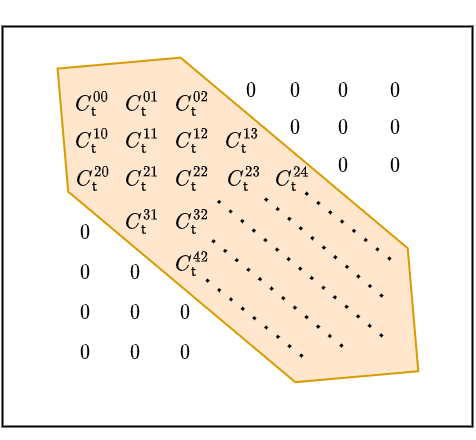
\includegraphics[width=9cm]{images/banded-matrix.drawio.png}
\caption{An illustration of a banded covariance matrix with a bandwidth of 2.}
\label{fig:banded-matrix}
\end{figure}

The extra detail that's also needed here is to consider how we encode a 2-dimensional spatial process into our state vector, and how the elements of the resulting state vector might be correlated to one another depending on their spatial proximity. If we start with a Markovian Gaussian random field, we can derive the Mat\'{e}rn kernel over these spatial coordinates in order to correlate the state vectors in such a way.